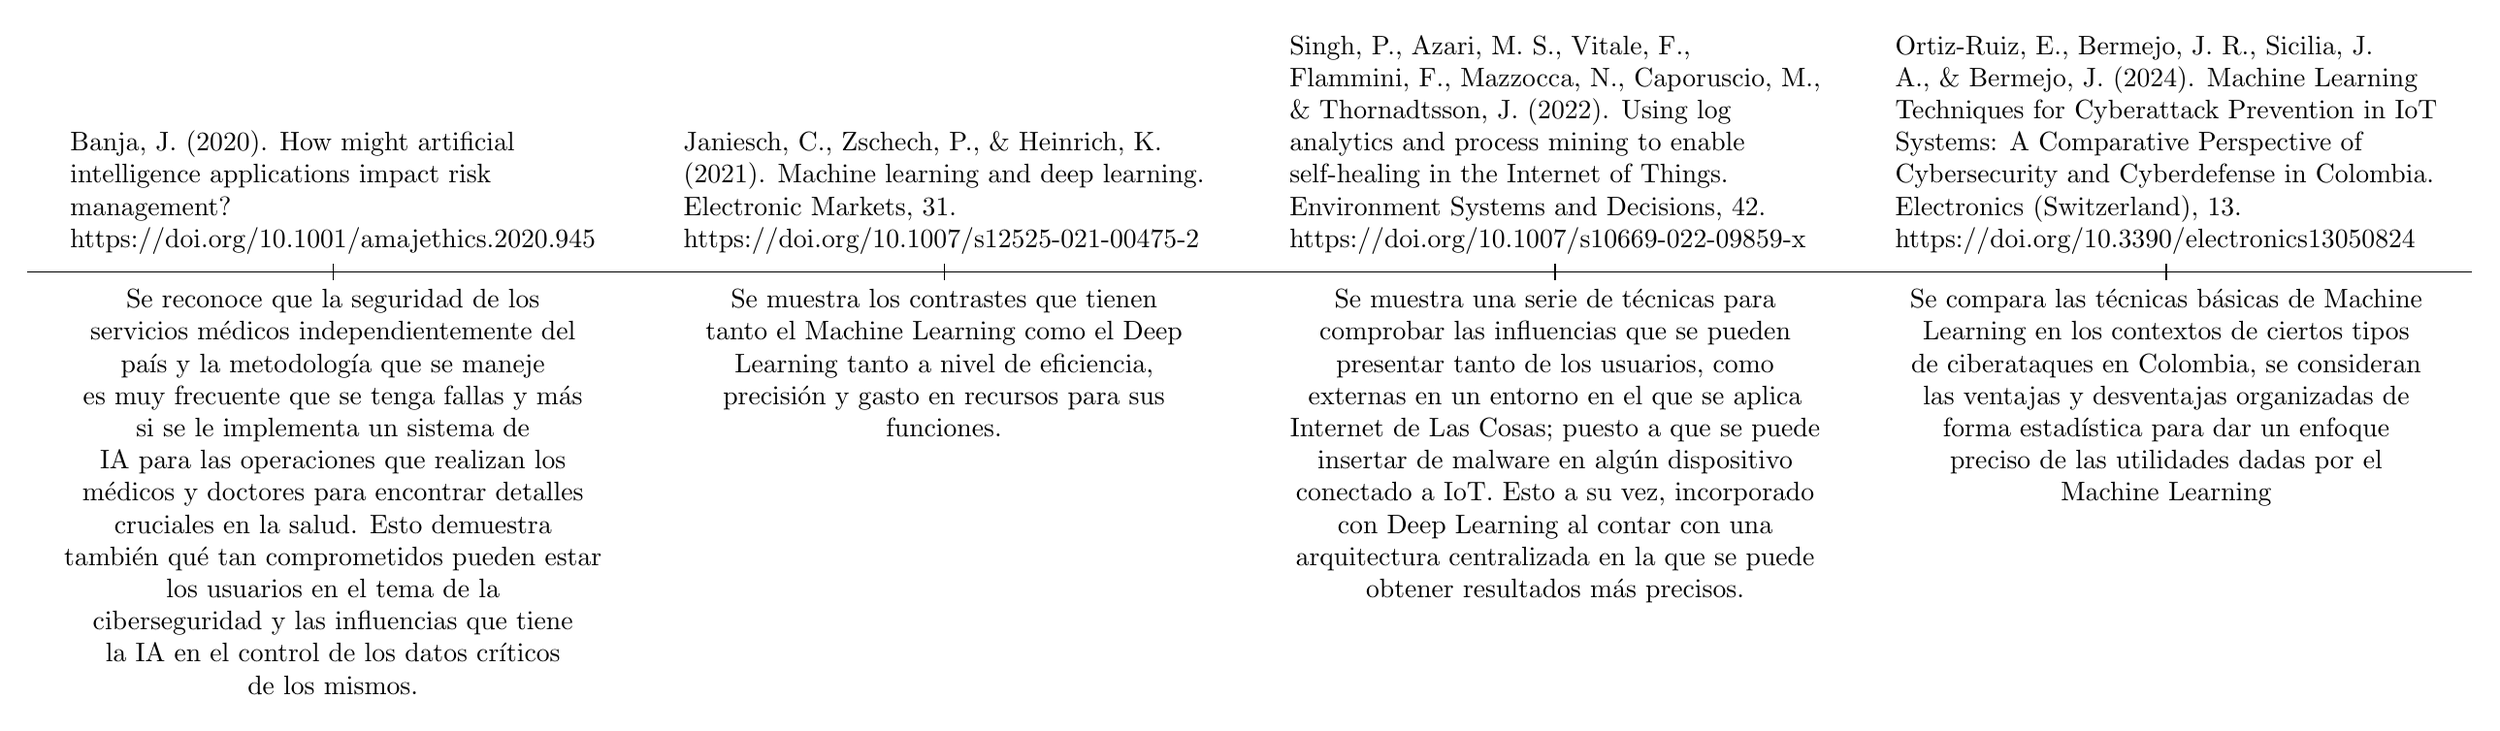
\begin{tikzpicture}
% draw a horizontal line
\draw (0,0) -- (32,0);
% draw vertical lines
\foreach \x in {4,12,20,28}
\draw (\x cm,3pt) -- (\x cm,-3pt);

% draw nodes to add events
\draw (0,0) -- (32,0);
% draw vertical lines
\foreach \x in {4,12,20,28}
\draw (\x cm,3pt) -- (\x cm,-3pt);

% draw nodes to add events
\draw (4,0) node[below=3pt, align=center] {
  Se reconoce que la seguridad de los \\
  servicios médicos independientemente del \\
  país y la metodología que se maneje \\
  es muy frecuente que se tenga fallas y más \\
  si se le implementa un sistema de \\
  IA para las operaciones que realizan los \\
  médicos y doctores para encontrar detalles \\
  cruciales en la salud. Esto demuestra \\
  también qué tan comprometidos pueden estar \\
  los usuarios en el tema de la \\
  ciberseguridad y las influencias que tiene \\
  la IA en el control de los datos críticos \\
  de los mismos.
} 
node[above=3pt, align=left] {
  Banja, J. (2020). How might artificial\\
  intelligence applications impact risk\\
  management?\\
  https://doi.org/10.1001/amajethics.2020.945
};
\draw (12,0) node[below=3pt, align=center] {
  Se muestra los contrastes que tienen \\
  tanto el Machine Learning como el Deep \\
  Learning tanto a nivel de eficiencia, \\
  precisión y gasto en recursos para sus \\
  funciones.
} node[above=3pt, align=left] {
  Janiesch, C., Zschech, P., \& Heinrich, K.\\
  (2021). Machine learning and deep learning.\\
  Electronic Markets, 31.\\
  https://doi.org/10.1007/s12525-021-00475-2
};
\draw (20,0) node[below=3pt, align=center] {
  Se muestra una serie de técnicas para \\
  comprobar las influencias que se pueden \\
  presentar tanto de los usuarios, como \\
  externas en un entorno en el que se aplica \\
  Internet de Las Cosas; puesto a que se puede \\
  insertar de malware en algún dispositivo \\
  conectado a IoT. Esto a su vez, incorporado \\
  con Deep Learning al contar con una \\
  arquitectura centralizada en la que se puede \\
  obtener resultados más precisos.
} node[above=3pt, align=left] {
  Singh, P., Azari, M. S., Vitale, F.,\\
  Flammini, F., Mazzocca, N., Caporuscio, M.,\\
  \& Thornadtsson, J. (2022). Using log\\
  analytics and process mining to enable\\
  self-healing in the Internet of Things.\\
  Environment Systems and Decisions, 42.\\
  https://doi.org/10.1007/s10669-022-09859-x
};
\draw (28,0) node[below=3pt, align=center] {
  Se compara las técnicas básicas de Machine \\
  Learning en los contextos de ciertos tipos \\
  de ciberataques en Colombia, se consideran \\
  las ventajas y desventajas organizadas de \\
  forma estadística para dar un enfoque \\
  preciso de las utilidades dadas por el \\
  Machine Learning
} node[above=3pt, align=left] {
  Ortiz-Ruiz, E., Bermejo, J. R., Sicilia, J.\\
  A., \& Bermejo, J. (2024). Machine Learning\\
  Techniques for Cyberattack Prevention in IoT\\
  Systems: A Comparative Perspective of\\
  Cybersecurity and Cyberdefense in Colombia.\\
  Electronics (Switzerland), 13.\\
  https://doi.org/10.3390/electronics13050824
};
\end{tikzpicture}
